%% 
%% Copyright 2019 Elsevier Ltd
%% 
%% This file is part of the 'CAS Bundle'.
%% --------------------------------------
%% 
%% It may be distributed under the conditions of the LaTeX Project Public
%% License, either version 1.2 of this license or (at your option) any
%% later version.  The latest version of this license is in
%%    http://www.latex-project.org/lppl.txt
%% and version 1.2 or later is part of all distributions of LaTeX
%% version 1999/12/01 or later.
%% 
%% The list of all files belonging to the 'CAS Bundle' is
%% given in the file `manifest.txt'.
%% 
%% Template article for cas-sc documentclass for 
%% single column output.

%\documentclass[a4paper,fleqn,longmktitle]{cas-sc}
\documentclass[a4paper,fleqn]{cas-sc}

%\usepackage[numbers]{natbib}
%\usepackage[authoryear]{natbib}
% \usepackage[authoryear,longnamesfirst]{natbib}
\usepackage[authoryear]{natbib}
\usepackage[showframe]{geometry}

\usepackage{graphicx}
\usepackage{amsmath}
\usepackage{algorithm}% http://ctan.org/pkg/algorithms
\usepackage{algpseudocode}% http://ctan.org/pkg/algorithmicx
\usepackage{amssymb} % for empty set
\usepackage{booktabs}
\usepackage{tabularx}
\usepackage{array}
\usepackage{float}
\usepackage[caption=true]{subfig}


\algrenewcommand\algorithmicrequire{\textbf{Input:}}
\algrenewcommand\algorithmicensure{\textbf{Output:}}
\let\emptyset\varnothing
\usepackage[section]{placeins}
\usepackage[caption=false]{subfig}
\usepackage{capt-of}

%%%Author macros
\def\tsc#1{\csdef{#1}{\textsc{\lowercase{#1}}\xspace}}
\tsc{WGM}
\tsc{QE}
\tsc{EP}
\tsc{PMS}
\tsc{BEC}
\tsc{DE}
%%%

\begin{document}
\let\WriteBookmarks\relax
\def\floatpagepagefraction{1}
\def\textpagefraction{.001}
\shorttitle{Preprint submitted to Elsevier}
\shortauthors{Da Lei et~al.}
%\begin{frontmatter}

\title [mode = title]{Role discovery in dynamical passenger flow networks}                      
% \tnotemark[1,2]

% \tnotetext[1]{This document is the results of the research
%   project funded by the National Science Foundation.}

% \tnotetext[2]{The second title footnote which is a longer text matter
%   to fill through the whole text width and overflow into
%   another line in the footnotes area of the first page.}



% \author[1]{Da Lei}[type=editor,
%                         auid=000,bioid=1,
%                         % prefix=Sir,
%                         role=Researcher,
%                         o 
% 6
% rcid=0000-0001-7511-2910]
\author[1,2,3]{Da Lei}[%
]
% \cormark[1]
% \fnmark[1]
% \ead{cvr_1@tug.org.in}
% \ead[url]{www.cvr.cc, cvr@sayahna.org}

% \credit{Conceptualization of this study, Methodology, Software}

\address[1]{Jiangsu Key Laboratory of Urban ITS, Southeast University, Nanjing 211189, China}
\address[2]{Jiangsu Province Collaborative Innovation Center of Modern Urban Traffic Technologies, Southeast University, Nanjing 211189, China}
\address[3]{School of Transportation, Southeast University, Nanjing 211189, China}

\author[1,2,3]{Xuewu Chen}[%
]
\cormark[1]

\author
[4]
{Long Cheng}
% \cormark[2]
% \fnmark[1,3]
% \ead{rishi@stmdocs.in}
% \ead[URL]{www.stmdocs.in}

\address[4]{Department of Geography, Ghent University, Krijgslaan 281 S8, Ghent 9000, Belgium}

\address[5]{School of Civil Engineering and Transportation, South China University of Technology, Guangzhou, 510641, China}

\author%
[5]
{Lin Zhang}[%
]

\author%
[4]
{Frank Witlox}[%
]


\cortext[cor1]{Corresponding author}
% \cortext[cor2]{Principal corresponding author}
% \fntext[fn1]{This is the first author footnote. but is common to third
%   author as well.}
% \fntext[fn2]{Another author footnote, this is a very long footnote and
%   it should be a really long footnote. But this footnote is not yet
%   sufficiently long enough to make two lines of footnote text.}

% \nonumnote{This note has no numbers. In this work we demonstrate $a_b$
%   the formation Y\_1 of a new type of polariton on the interface
%   between a cuprous oxide slab and a polystyrene micro-sphere placed
%   on the slab.
%   }

\begin{abstract}
In this paper, we proposed a new approach to automatically extract the role of a station in dynamical public transport (PT) flow networks based on the emerging role discovery method in network science. With notions of dynamical graph and edge, we first constructed dynamical PT flow networks using smart card data from Nanjing bikesharing agencies. We then developed a dynamical algorithm to compute the structural flow features of nodes from passenger flow networks recursively. We conducted Non-negative Matrix Factorization (NMF) to extract the role memberships from the derived structural feature matrix and interpret each role in terms of measurements with practical value. Network hubs and potential service bottlenecks are identified and named according to their operating characteristics and dynamics. Moreover, the proposed method unveils day-to-day and within-day role dynamics of PT stations over time. The analysis results contribute to a better understanding of the interplay among stations in the network. The identification of roles also provides insights for transit agencies to improve service quality.
\end{abstract}

\begin{keywords}
role extraction \sep smart card data \sep unsupervised learning \sep public transportation \sep network dynamics \sep transit flow patterns
\end{keywords}


\maketitle

\section{Introduction}
Public transportation has been considered to be an effective solution to the increasing challenges of traffic congestion in cities. Understanding the dynamics of PT networks is of importance for the evidence-based PT service planning and management. With the rapid development of urbanization and technology, it is challenging for us to explore the dynamics of PT networks as they become much larger and more complex, allied with our increasing accessibility to large-scale automatically-collected data sources like smart card (SC) data. Network science provides us an abstraction for quantitatively analyzing the collective dynamics accounting for the interactions among components in networks across a broad set of disciplines, including transport, biology, information, social sciences \citep{de2004fluctuations,vogels2005neural,tyson2001network,coviello2006network,snijders2010introduction}. Over the past decades, we have seen a considerable amount of network studies on PT systems \citep{wu2004urban,ping2006topological,lu2007complexity,qing2013space,zhang2019quantitatively}. Most of them, however, were conducted by network researchers rather than transportation researchers and engineers. Consequently, these studies often focused on investigating the topological complexity of PT networks without in-depth insights into PT-related attributes, leading to claims by transport scientists that these works only make very limited contributions to our understanding of the dynamics of PT networks (see detailed discussion in \cite{luo2019integrating}). Moreover, most of the existing literature on the application of network to PT systems examined the time-varying network characteristics at a long granularity of time, resulting in the growing concern about the utility of network sciences on PT systems as it can not capture the day-to-day and within-day dynamical network performance \citep{leng2014evaluating,ding2015complex,zhu2016evolution,cats2017topological}. 

In the field of PT research, exploring spatial-temporal travel behavior (or passenger flow pattern) has long been a focus for decades. One class of these studies relied on conventional travel survey data\citep{recker1985travel,hanson1988systematic,pas1995intrapersonal,joh2002activity,susilo2005analysis}. For the thorough discussion about major drawbacks of applying travel survey data to analyze travel behaviors, we refer to \cite{tao2014examining}. Given the increasing availability of automatically-collected data sources like smart card data, more academic attention has been paid to spatial-temporal travel behavior analysis exploiting emerging data sources(\citep{morency2007measuring,ortega2013classification,6981952,ouyang2018passenger}). Both types of data-based studies mainly offer insights into the dynamical characteristics of travel behavior of individuals or passenger flows rather than the PT networks and its primary components (e,g. stations and routes). For instance, \cite{ma2013mining} applied a DBSCAN algorithm and identified commuting patterns of transit passengers in Beijing. They also conducted partitioning algorithms to compute travel pattern regularity and recognized frequent transit passengers. The transport community has paid rare attention to investigate the dynamics of PT networks. Traditional dynamic transportation models only reveal some of the PT network's time-evolving characteristics, such as departure time distribution and passenger cost dynamics, from their simulated results instead of travel flow patterns in the real world \citep{hamdouch2011schedule,ma2011hybrid,nuzzolo2012schedule,yao2013modeling}. \cite{yap2019shall} identified critical network hubs to address the challenge of solving the Timetable Synchronization Problem(TSP) for Large PT networks. They first perform DBSCAN to determine the spatial boundaries of transfer locations. Then, network hubs are identified by the Herfindahl- Hirschman Index (HHI) based on the volume of transfer flows directly linked to stations.

\begin{figure}
  \begin{minipage}[b]{0.55\textwidth}
     \centering
     \noindent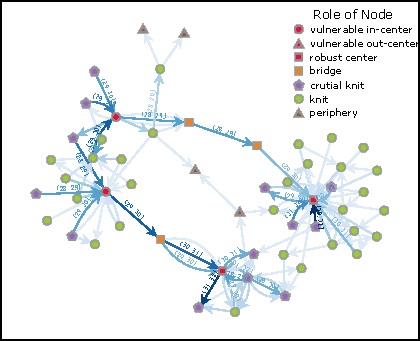
\includegraphics[width=0.95\linewidth]{figs/notion_explanation.pdf}
     \caption{An illustration of role identification from the \newline case study of the dynamical bikesharing network in Nanjing.\newline Roles are interpreted with measurements concerning daily\newline operation. We will discuss it later in details}\label{fig:notion_explanation}
  \end{minipage}\hfill
  \begin{minipage}[b]{0.45\textwidth}
     \centering
     \noindent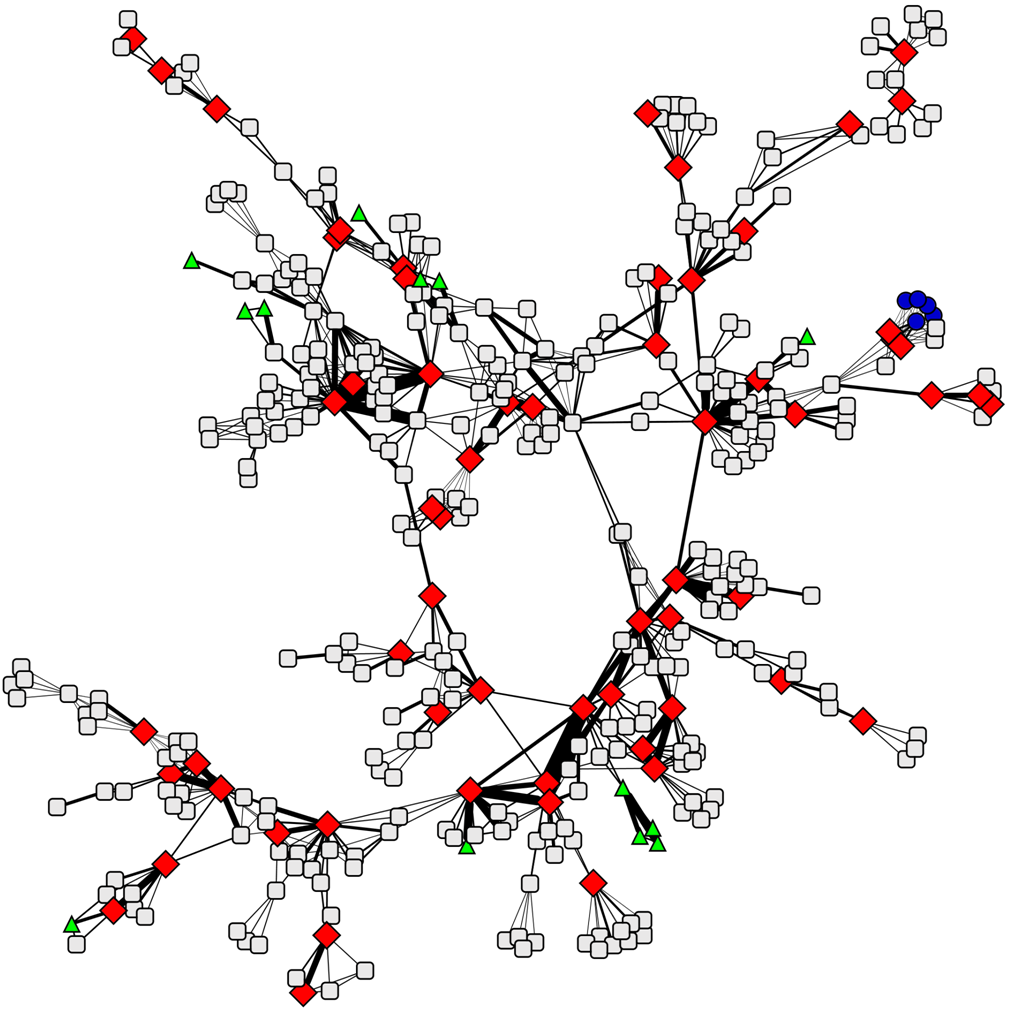
\includegraphics[width=0.95\linewidth]{figs/co_author_role.png}
     \caption{A snapshot of role identification in a \newline large co-authorship network\citep{henderson2011s}}\label{fig:coauthorrole}
  \end{minipage}
\end{figure}

The aforementioned extant literature from the transportation community generally overlooks the topological importance of stations in PT networks. The notion of topological (structural) importance was first introduced by sociologists in the early 1950s \citep{parsons1951illness,merton1968social}. They also defined "role" as groups of nodes with structural equivalence. In other words, nodes of the same role have the same topological importance. In recent decades, 
role discovery in networks has been of interest to scholars from different fields, including communication \citep{mahadevan2006internet}, biology \citep{varki1993biological,helenius2004roles}, online sociology \citep{scripps2007node}. For example, \cite{henderson2012rolx} proposed a feature-based role discovery method to extract roles from a co-authorship network. For the history and recent development of role discovery techniques we refer to \cite{rossi2014role}. "Role" is an overgeneralized word in an extensive set of disciplines on which the contextual interpretation of the concept varies according to their differences in system characteristics. For instance, a co-authorship network can be approximated as a static graph since its variation is limited over a considerable span of time. In contrast, the domain of transportation involves a highly dynamical network where temporal information is crucial, for example, a PT passenger network. Thus, the roles identified in the bikesharing ridership network shown in \hyperref[fig:notion_explanation]{Figure.~\ref{fig:notion_explanation}} significantly differ from those of the co-authorship presented in \hyperref[fig:coauthorrole]{Figure.~\ref{fig:coauthorrole}}, even with the consensus on the notion of structural equivalence. Although the temporal information in graphs has received increasing attention from the academic community, most existing studies can only partially capture it by approximating the dynamical network using a sequence of static network snapshots \citep{rossi2012role, rossi2013modeling, saha2018models}. Moreover, we noticed that a few recent studies had developed temporal random walk-based approaches to address the problem of node embedding in dynamical networks (typically a communication network) consisting of a sequence of edges with single unique timestamps \citep{beres2019node,lee2020dynamic}. However, such methods are still not feasible for dynamical PT passenger networks since a passenger flow generally has a start time and end time.

To this end, there is a compelling need for emerging techniques to capture the role of PT components in dynamical networks, unveiling the time-varying interplay among them and explore role dynamics and behavioral patterns.
Inspired by the existing role discovery studies, we aim to propose a role extraction framework for dynamical PT flow networks to understand how the characteristics of individual nodes (stations) change over time by integrating network science and domain knowledge in transportation engineering. To our best knowledge, there are no studies reported that utilizing role discovery techniques to investigate dynamics in PT networks and even other general transportation networks. Our primary contributions are (1) filling the current research gap and providing an in-depth understanding of the within-day and day-to-day flow and topological characteristics of PT stations; (2) identify important nodes and potential service bottlenecks over time for policy-making and service management adaption. Our approach is interpretable, feasible to similar transport systems where the O-D matrix is available and lends itself to intuitive visualizations.

The remainder of the paper is structured as follows: \hyperref[Methodology]{Section.\ref{Methodology}} introduces the methods utilized in this study, including the dynamical structural feature extraction, role clustering based on the non-negative matrix factorization (NMF), automation of role number selection and role interpretation approaches. In \hyperref[case_study]{Section.\ref{case_study}}, one case study based on the dynamical bikesharing ridership flow network are described. \hyperref[conclusion]{Section.\ref{conclusion}} concludes the study with insights derived from modeling, analysis results, current limitations, and future research directions.

\section{Methodology}\label{Methodology}
For the remainder of the paper, we introduce algorithms, indices, sets, network measurements, and variables used in this study. Furthermore, we introduce the following definitions as preliminaries for the following analysis.

\textit{\textbf{Definition 1 Dynamical Edge:}} A dynamical edge (or temporal edge) $e_=\left(u, v, t_{s},t_{e}\right)$ is defined as a directed edge with timestamp attributes, where $u$ and $v$ are the origin and destination nodes respectively, and $t_{s},t_{e}$ are the corresponding start and end timestamps of $e$. Timestamps denote the start and end periods instead of exact time points. In this study, each $e$ represents a passenger flow from the origin station $u$ to the destination $v$ (starting from $t_{s}$ to $t_{e}$). Notice that $t_{s}=t_{e}$ is possible under our definition.

\textit{\textbf{Definition 2 Checking Window:}} To evaluate the dynamics of flows in the network in a duration of time, we define a checking window $T$ as a time period when the interplay among nodes happens.

\textit{\textbf{Definition 3 Dynamical Graph:}} A temporal graph or temporal network $G=(V,E)$ comprises a set of nodes $V$ and a temporal edge set $E=\{(u, v, t_{s},t_{e})|u,v\in V\}$. In the later case study, we split one day into 15-minute time intervals (96 intervals for one day). Daily travel transactions are then grouped into dynamical edges (flows) $e_=\left(u, v, t_{s},t_{e}\right)$ from which dynamical graphs are constructed. \hyperref[fig:d_graph_instance]{Figure.~\ref{fig:d_graph_instance}} shows an example of a dynamical graph within an hourly checking window $T$ starting from "2019-03-04 07:00:00" to "2019-03-04 08:00:00". Timestamp labels $<t_{s},t_{e}]$ on edges of the network denote the specific beginning and ending periods of each flow. For example, $<29,30]$ means that the corresponding passenger flow starts in the 29th interval ("07:00:00-07:15:00") and ends in the 30th  ("07:15:00-07:30:00"). \hyperref[fig:d_graph_instance]{Figure.~\ref{fig:d_graph_instance}} only presents a subgraph and timestamps on major streams for visual simplicity.

\begin{figure}[!htb]
  \centering
  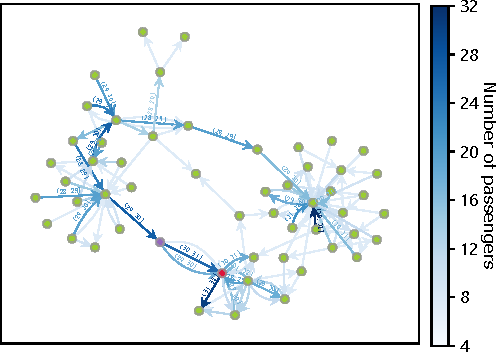
\includegraphics[width=0.7\textwidth]{figs/d_graph_instance.pdf}
  \caption{An instance of dynamical bikesharing passenger flow network (subgraph) in Nanjing. The checking window $T$ starts from 2019-03-04 07:00:00 to 2019-03-04 08:00:00. Dynamical edges with any of their timestamps lying within $T$ are presented in this figure.}\label{fig:d_graph_instance}
\end{figure}

\textit{\textbf{Definition 4 Egonet:}} The egonet of a target node $u$ consists of node u ("ego"), neighbors of $u$, and edges linked to $u$ and its neighbors. \hyperref[fig:real_ego_net]{Figure.~\ref{fig:real_ego_net}} presents the egonet of a target node $u$ from the network shown in \hyperref[fig:d_graph_instance]{Figure.~\ref{fig:d_graph_instance}}. Egonet has been utilized as a basis for extracting local structural attributes of complex networks in an extensive set of disciplines, including communication, social, and bioinformatics networks \citep{straits1996ego,edwards2009measures,yang2014egonet}.

\begin{figure}[!htb]
  \centering
  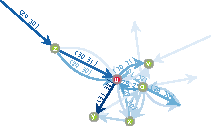
\includegraphics[width=0.5\textwidth]{figs/real_ego_net.pdf}
  \caption{An instance of a bikesharing-flow egonet of the target node $u$ within the checking window $T$.}\label{fig:real_ego_net}
\end{figure}

\subsection{Dynamical recursive feature extraction}
Node embedding, a process to encode nodes in a given network to a feature space (map nodes to feature matrix), is crucial for many graph-based data mining tasks such as link prediction and outlier detection. Here, we propose a novel node-embedding algorithm that recursively combines dynamical edges across the network via edges and produces regional flow features that capture topological information and flow dynamics, as shown in \hyperref[alg:alg1]{Algorithm.~\ref{alg:alg1}}. The algorithm is a modified version of the ReFeX algorithm first introduced by \cite{henderson2011s}. Starting from a feature initialization, the ReFex aggregates each node's neighboring attributes simultaneously in iterations to transmit information to each target node from its neighbors, neighbors' neighbors, etc. However, the original ReFeX algorithm, among many other node-embedding techniques, only applies to static networks. In reality, networks evolve over time with the changing number and weight of edges and nodes. Although the temporal information in graphs has received increasing attention from the academic community, most existing studies can only partially capture it by approximating the dynamical network using a sequence of static network snapshots \citep{rossi2012role, rossi2013modeling, saha2018models}. Moreover, we noticed that a few recent studies had developed temporal random walk-based approaches to address the problem of node embedding in dynamical networks (typically a communication network) consisting of a sequence of edges with single unique timestamps \citep{beres2019node,lee2020dynamic}. However, such methods are still not feasible for dynamical PT passenger networks since a passenger flow generally has a start time and end time. Our proposed DyReFex echoes the mechanism of the ReFeX but with an additional constraint that requires each aggregation to respect the arrival and departure time of passenger flows.

The initial features that seed the DyReFeX process include local and egonet features (together called neighborhood features), as shown in \hyperref[equ:bikesharing_base_feature]{Equation.~\ref{equ:bikesharing_base_feature}}. Local features ($W_{in}(u)$ and $W_{out}(u)$) are basically node degree measures but in the directed and weighted version for our case study of transit flow networks. Egonet features are computed for each node based on the node's egonet, including the total volume of within-egonet flows ($W_{in}^{ego}(u)$) and the volume of flows entering and leaving the egonet ($W_{out}^{ego}(u$). The set of initial features can be extended to seed the DyReFex for multi-layer networks (e.g., a multi-mode transit network) to capture the heterogeneity of edges/flows.


% $W_{in}(u) = w(e_{o,u}^{28,29}) + w(e_{v,u}^{28,29})$
% $W_{out}(u) = w(e_{u,x}^{29,30})$
% $W_{in}^{ego}(u) = w(e_{o,v}^{29,29}) + w(e_{o,u}^{28,29})$
% $W_{out}^{ego}(u) = w(e_{p,v}^{28,29}) + w(e_{o,q}^{29,30}) + w(e_{x,y}^{29,30})$
% $F_{u}^{29} = \{W_{in}(u), W_{out}(u), W_{in}^{ego}(u), W_{out}^{ego}(u)\}$

% $sum_{in}(u) = w(e_{z,u}^{29,30})F_{z}^{29} + w(e_{x,u}^{29,30})F_{x}^{29}$
% $sum_{out}(u) = w(e_{u,x}^{29,30})F_{x}^{30}$
% $avg_{in}(u) = \frac{1}{N_{u}^{in}}sum_{in}(u)$
% $avg_{out}(u) = \frac{1}{N_{u}^{out}}sum_{out}(u)$
% $F_{u}^{31} = \{sum_{in}(u), sum_{out}(u), avg_{in}(u), avg_{out}(u)\}$
% $sum_{in}(u) = w(e_{z,u}^{30,31})F_{z}^{30} + w(e_{v,u}^{29,31})F_{v}^{29}
% sum_{out}(u) = w(e_{u,x}^{30,31})F_{v}^{31}$

\begin{equation}
F_{u}^{0} = \{W_{in}(u), W_{out}(u), W_{in}^{ego}(u), W_{out}^{ego}(u)\}
\label{equ:bikesharing_base_feature}
\end{equation}

where $F_{u}^{t_{0}}$ means the initial flow feature vector of node $u$. $W_{in}(u)$ and $W_{out}(u)$ are the weighted in/out degrees of node $u$, which represent passenger flow arriving at/ alighting from node $u$, respectively.

We utilize simple functions, summation and average (presented in \hyperref[equ:summation_in]{Equation.~\ref{equ:summation_in}} to \hyperref[equ:avg_out]{Equation.~\ref{equ:avg_out}}), as the aggregation methods. However, the DyFeReX is not restricted to these two functions.

\noindent\begin{minipage}{.5\linewidth}
\begin{equation}
sum_{in}(u) = \sum\limits_{v\in N_{u}^{in}}w(e_{v,u}^{t_{s},t_{e}})F_{v}^{t_{s}}
\label{equ:summation_in}
\end{equation}
\end{minipage}%
\begin{minipage}{.5\linewidth}
\begin{equation}
sum_{out}(u) = \sum\limits_{v\in N_{u}^{out}}w(e_{u,v}^{t_{s},t_{e}})F_{v}^{t_{s}}
\label{equ:summation_out}
\end{equation}
\end{minipage}

\noindent\begin{minipage}{.5\linewidth}
\begin{equation}
avg_{in}(u) = \frac{1}{|N_{u}^{in}|}sum_{in}(u)
\label{equ:avg_in}
\end{equation}
\end{minipage}%
\begin{minipage}{.5\linewidth}
\begin{equation}
avg_{out}(u) = \frac{1}{|N_{u}^{out}|}sum_{out}(u)
\label{equ:avg_out}
\end{equation}
\end{minipage}

where $e_{u,v}^{t_{s},t_{e}}$ denotes the dynamical edge from $u$ at $t_{s}$ to $v$ at $t_{s}$ and node $v$ is called a in-neighbor of $u$; the node $v$ of an edge $e_{v,u}^{t_{s},t_{e}}$ is called a out-neighbor of node $u$; $w(\cdot)$ measure the weight/volume of the dynamical edge; $F_{v}^{t_{s}}$ is the feature set of $v$ at $t_{s}$; $N_{u}^{in}$ and $N_{u}^{out}$ represent the in-neighbor and out-neighbor sets of node $u$.


\begin{algorithm}[!htb]
    \caption{\textbf{DyReFeX}}
    \label{alg:ALG1}
    \begin{algorithmic}
    \Require The dynamical network $G$ and the checking window $T$.
    \Ensure The recursive feature set $\textbf{F} = F_{nodes}$ of all nodes within $T$
    
    \Procedure {MainProcess}{$G$, $T$} 
        \State $t\gets$ the first interval in $T$
        \State $F^{t}\gets$ computer initial features for all nodes
        \For{$t$ \textbf{in} $T$}
        \ForAll{nodes $u$ in $G$}
        \State $N_{u}^{in}\gets$\textsc{GetInNeighbors}($G, u$) at $t$
        \State $N_{u}^{out}\gets$\textsc{GetOutNeighbors}($G, u$) at $t$
        \State $F_{u}^{t+1}\gets\{sum_{in}(u), sum_{out}(u), avg_{in}(u), avg_{out}(u)\}$ for $t_{s} == t$
        \EndFor
        \State  $F^{t+1}\gets$ $F_{u}^{t+1}$ for $u\in G$
        \State $t=t+1$
        \EndFor
    \EndProcedure
    \end{algorithmic}\label{alg:alg1}
\end{algorithm}

\begin{figure}[!htb]
  \centering
  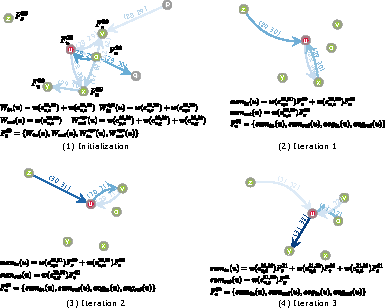
\includegraphics[width=0.8\textwidth]{figs/iteration_ins.pdf}
  \caption{The feature extraction process for node $u$. The final output feature matrix for node $u$ within the checking window $T$ is $F_{u} = \{F_{u}^{29}, F_{u}^{30}, F_{u}^{31}, F_{u}^{32}\}$}\label{fig:iteration_ins}
\end{figure}

The final output of \hyperref[alg:alg1]{Algorithm.~\ref{alg:alg1}} is a feature matrix $\textbf{F}\in \mathbb{R}^{n\times f}$ where $n$ is the number of nodes and $f$ is the number of features. To capture the within-day and day-to-day variability of structural roles for nodes, we should have multiple checking windows in a given day and employ the DyReFeX to consecutive daily dynamical graphs. If we set a checking window every half hour for $d$ days, the dimension of $\textbf{F}$ should be $\textbf{F}\in \mathbb{R}^{48dn\times f}$. \hyperref[fig:iteration_ins]{Figure.~\ref{fig:iteration_ins}} presents a concrete example of the DyReFex of node $u$ based on the dynamical graph shown in \hyperref[fig:d_graph_instance]{Figure.~\ref{fig:d_graph_instance}} and \hyperref[fig:real_ego_net]{Figure.~\ref{fig:real_ego_net}}. The start and end intervals do not need to be consecutive in the recursive feature extraction process. For example, $e_{v,u}^{29,31}$ shown in Iteration 2 in \hyperref[fig:iteration_ins]{Figure.~\ref{fig:iteration_ins}} is valid. To ensure the output vector $F_{u}^{31}$'s dimension is 64 in Iteration 2, we extend the feature vector $F_{v}^{29}$ related to $e_{v,u}^{29,31}$ with zeros to increase the dimension of $F_{v}^{29}$ from 4 to 16. The length and number of checking window T, together with the length of iteration step (interval) in the feature extraction procedure, will determine the dynamical scale of the observation. However, there is a trade-off between dynamics granularity and computation cost.

\subsection{Role extraction}
In the last subsection, we proposed an effective feature learning algorithm for automatically converting the graph data into a robust set of features that capture topological information of PT passenger flow networks. This subsection focuses on assigning nodes with similar structural features to the same role. In other words, this subsection is to conduct a clustering.  A variety of ways can be applied to complete the role assignment task, which can be grouped into two categories: hard and soft role assignment methods. Hard role assignment means each node can only be allowed in one role/cluster \citep{nowicki2001estimation,batagelj2004generalized}. Typical hard role assignment includes clustering approaches such as k-means, k-medoids \citep{zhu2005semi,berkhin2006survey}. In contrast to the hard role assignment, soft role assignment allocates nodes to multiple groups \citep{airoldi2008mixed, fu2009dynamic}. Classical soft role assignment comprises Principal Component Analysis (PCA) , Singular Value Decomposition (SVD) , spectral decomposition , Non-negative Matrix Factorization (NMF) et cetera \citep{wold1987principal,golub1971singular,partyka1999interpretational,lee1999learning}. 

In this study, we employed NMF to extract roles from the regional feature matrix we obtained in the last step because NMF is efficient even for a large dataset. Its non-negative decomposed matrix makes it easier for us to interpret roles than its most competitors. Moreover, NMF gives us more flexibility. The output delivers a role membership distribution in a continuous manner, while such a soft role assignment could turn into a hard one by assigning each node to a specific role with the highest role membership. Given the feature matrix $\textbf{F}\in \mathbb{R}^{n\times f}$, we want to construct a low-rank approximation $\textbf{WH} \approx \textbf{F}$ where each row of $\textbf{
W}\in \mathbb{R}^{n\times r}$ denotes a node's role membership and each column of $\textbf{
H}\in \mathbb{R}^{r\times f}$ expresses the contribution of each role to each regional feature.The two non-negative matrices \textbf{W} and \textbf{H} minimize the following objective function presented in \hyperref[equ:bikesharing_base_feature]{Equation.~\ref{equ:NMF_obj_fun}}.

\begin{equation}
f(\textbf{W},\textbf{H}) = \frac{1}{2}\mid\mid\textbf{F} - \textbf{WH}\mid\mid^{2}
\label{equ:NMF_obj_fun}
\end{equation}

$\mid\mid\cdot\mid\mid^{2}$ represents the divergence function (or objective function) for measuring the distance between \textbf{F} and the dot product \textbf{WH}. A few classical choices for $\mid\mid\cdot\mid\mid^{2}$ are Frobenius norm and Kullback-Leibler (KL) divergence, among others. Due to the non-convexity of the objective function of NMF, the optimal solution is usually approximated by iterative update algorithms such as Multiplicative Update (MU) \citep{lee1999learning}, Coordinate Descent (CD) \citep{wright2015coordinate}. NMF is not tied to any specific objective function and solver setting. The setting choices for the NMF model are flexible according to the application and computational limits. In our case studies, we found that NMF using KL-divergence with MU solver is generally a proper NMF-based model setting for exploring PT passenger flow networks in terms of runtime, accuracy and simplicity.

\subsection{Automating model selection}
Notice that the number of roles $r$ in NMF needs to be predefined. It is impractical to select r manually each time when we want to extract roles from different network data. Therefore, an automatic role number selection mechanism is necessary for us to make sure the whole framework of our study is nonparametric and automated. In past decades, many methods have been proposed for deciding the proper number of roles (or clusters) among which Akaike's information criterion (AIC) and Minimum Description Length (MDL) are two reliable approaches from the literature of statistics and information theory \citep{akaike1974new, rissanen1978modeling, cook2007graph, grunwald2007minimum, rossi2014role}. 

\hyperref[alg:alg2]{Algorithm.~\ref{alg:alg2}} shows the automation of an MDL-based role number selection with KL-divergence. The error of our model $\mu$ can be split into two parts: (1) the error of role extraction (NMF in this study) $\varepsilon_{extraction}$ and (2) the description cost $\eta$. Intuitively, the growing number of roles $r$ raises model complexity, thus increasing our description cost but decreasing role extraction errors, and vice versa. Basically, \hyperref[alg:alg2]{Algorithm.~\ref{alg:alg2}} is trying to seek a balance between these two types of errors. \hyperref[equ:extractionerror]{Equation.~\ref{equ:extractionerror}} represents the KL-divergence described role extraction error $\varepsilon_{extraction}$ (see details in \cite{yang2011kullback}). The description cost is generally defined as the number of \textit{bits} in the field of information theory. A \textit{bit} is a basic unit for storing information. For example, a 16-bit integer can stand for $2^{16}$ (65,536) distinct values. The total description cost $\eta$ for $\textbf{F}\in \mathbb{R}^{n\times f}$ and 
$\textbf{
W}\in \mathbb{R}^{n\times r}$ is formulated in \hyperref[equ:descriptioncost]{Equation.~\ref{equ:descriptioncost}} in terms of bits where $b$ is the average bits per value. Typically, $b=\log_{2}{M}$ where $M$ is the total number of distinct values in matrices \textbf{W} and \textbf{H}. For example, $b = 16$ if there are 65,536 different values in \textbf{W} and \textbf{H}. \hyperref[fig:kl_divergence_role_intepretation]{Figure.~\ref{fig:kl_divergence_role_intepretation}} presents  the variation of role extraction error and description cost as the number of roles increases.The model error $\mu$ is minimized when the number of roles equals 7 in the dynamical bikesharing flow network. 


\begin{equation}
\varepsilon_{extraction} = \sum\limits_{ij}(\textbf{F}_{ij}\text{log}\frac{\textbf{F}_{ij}}{(\textbf{WH})_{ij}} + (\textbf{WH})_{ij} - \textbf{F}_{ij})
\label{equ:extractionerror}
\end{equation}

\begin{equation}
\eta = br(n + f)
\label{equ:descriptioncost}
\end{equation}

\begin{algorithm}[!htb]
    \caption{\textbf{Role Number Selection}}
    \label{alg:ALG2}
    \begin{algorithmic}
    \Require The recursive feature set  $\textbf{F}$.
    \Ensure The optimal role number $r$.
    \State \textit{minerror}$\gets \infty$
    \State \textit{failure}$\gets 0$
    \State \textit{trails}$\gets \theta$
    \For{$r=1$ \textbf{to} min($n, f$)}
    \State$\varepsilon_{extraction} , \eta\gets  \;$NMF(\textbf{F}, $r$) with KL-divergence using MDL criterion
    \State$\mu = \varepsilon_{extraction} + \eta$
        \If{$\mu < minerror$ }
            \State \textit{minerror} $\gets \mu$
        \Else
            \State $\textit{failure} \gets \textit{failure}+1$
        \EndIf
        \If{$\textit{failure} \geq \textit{trails}$}
            \State return $\textbf{W}, \textbf{H} \gets \;$NMF(\textbf{F}, $r$)
        \EndIf
    \EndFor
    \end{algorithmic}\label{alg:alg2}
\end{algorithm}

\begin{figure}[!htb]
  \centering
  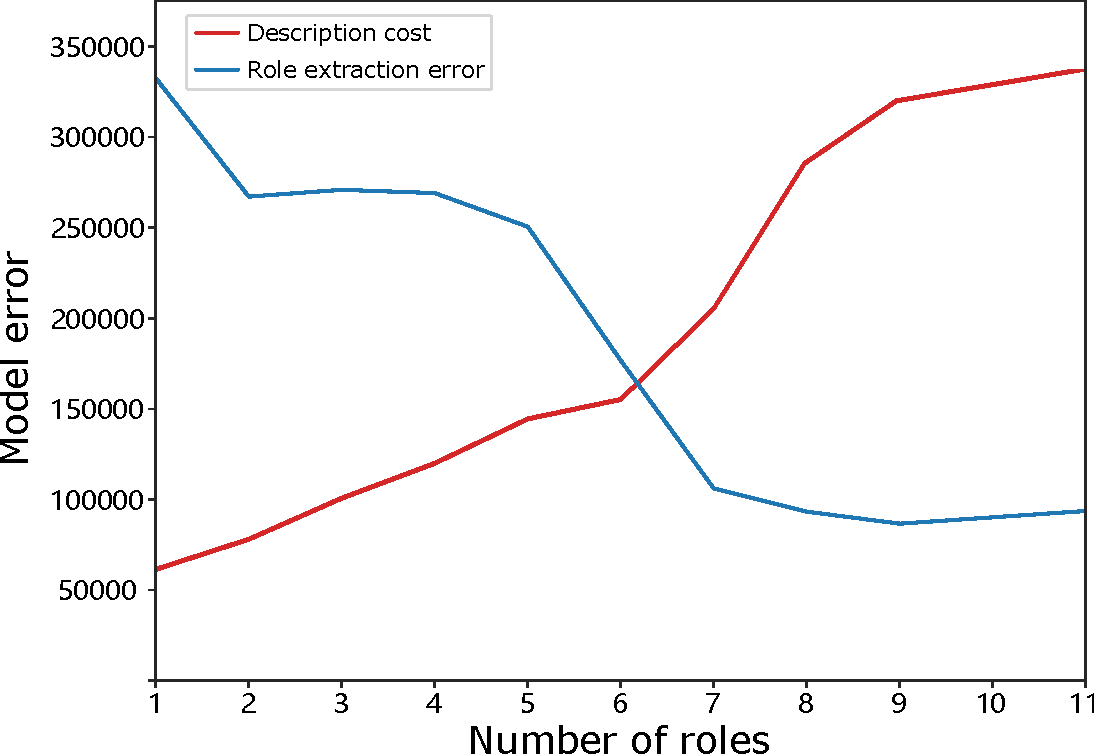
\includegraphics[width=0.6\textwidth]{figs/kl_divergence_role_intepretation.pdf}
  \caption{Model error in bits with an increasing number of roles.}\label{fig:kl_divergence_role_intepretation}
\end{figure}


\subsection{Role interpretation methods}\label{role_inter_method}
We interpret the roles based on a set of measurements capturing flow dynamics and topological information. The roles are rendered using the dynamic role memberships matrix $\textbf{W}\in \mathbb{R}^{n\times r}$ we derived before and a node measurement matrix $\textbf{M}\in \mathbb{R}^{n\times m}$ to calculate a non-negative matrix $\textbf{C}\in \mathbb{R}^{r\times m}$ (such that $\textbf{WC} \approx \textbf{M}$) presenting role contributions. For the bikesharing network, the first type of node measurements aims to evaluate service dynamics, including flow balance rate (\hyperref[equ:balance_rate]{Equation.~\ref{equ:balance_rate}}), entropy rates of full and empty stations (\hyperref[equ:entropy_limitation]{Equation.~\ref{equ:entropy_limitation}}), pass-through bike turnover rate (\hyperref[equ:pass_thro_turnover]{Equation.~\ref{equ:pass_thro_turnover}}). Then, we propose role affinity to evaluate the pair-wise topological relationship between roles. Intuitively, role affinity measures the average weighted distance from nodes of a specific role to nodes of another role. Role affinity is computed using \hyperref[alg:alg3]{Algorithm.~\ref{alg:alg3}}.

\begin{algorithm}[!htb]
    \caption{\textbf{Role Affinity Estimation}}
    \label{alg:ALG3}
    \begin{algorithmic}
    \Require The graph $G$; The hard role assignment matrix $\mathbf{W'}\in \mathbb{R}^{n\times r}$ where $n$ is the number of nodes and $r$ is the number of roles. Each node is assigned with only one role.
    \Ensure The role affinity matrix $\mathbf{Q}\in \mathbb{R}^{r\times r}$ within $T$.
    \State udpate each $w(e_{u,v}^{t_{s},t_{e}})\gets$ $\frac{w(e_{u,v}^{t_{s},t_{e}})}{\bar w(G)}$, $\bar w(G)$ is the average weight of $G$
    \State invert each $w(e_{u,v}^{t_{s},t_{e}})\gets$ $\frac{1}{w(e_{u,v}^{t_{s},t_{e}})}$
    \State shortest distance matrix $\mathbf{D}\gets$ apply Dijkstra's algorithm on $G$
    \State $\mathbf{Q}\gets$ compute the average shortest distance between each pair of nodes assigned with a specific role based on $\mathbf{D}$
    \State $\mathbf{Q}\gets$ normalize $\frac{1}{\mathbf{Q}}$ to rescale it into the range [0,1]
    \end{algorithmic}\label{alg:alg3}
\end{algorithm}

\begin{equation}
C_B(u) = \frac{|t|}{|T|}\sum\limits_{t\in T}\frac{\min(\sum\limits_{v\in N_{u}^{in}}w(e_{v,u}^{t_{s},t_{e}}),\sum\limits_{v\in N_{u}^{out}}w(e_{u,v}^{t_{s},t_{e}}))}{\max(\sum\limits_{v\in N_{u}^{in}}w(e_{v,u}^{t_{s},t_{e}}),\sum\limits_{v\in N_{u}^{out}}w(e_{u,v}^{t_{s},t_{e}}))}
\label{equ:balance_rate}
\end{equation}
\indent where $C_B(u)$ is the average flow balance rate within $T$; $t$ is the time interval; the component inside $\sum\limits_{t\in T}$ equals 1 when the in-flow and out-flow at $t$ is perfectly balanced.
\newline

The entropy rate of a station state sequence is presented in \hyperref[equ:entropy_limitation]{Equation.~\ref{equ:entropy_limitation}}. When a bikesharing station is full (no slots for returning bike) or empty (no available bikes), we assign a unique non-zero integer to the station state variable $X$ and a station state sequence $[1,2,3,0]$ means the bikesharing stop is full/empty in the first three intervals but recovered in the last interval. Entropy rate is often utilized to exhibit the degree of "surprise"/variability in an event sequence and has been applied in studies across multiple disciplines \citep{li2010blind,liu2011entropy,liu2013entropy,goulet2017measuring}. We employ entropy rates to measure the degree of resistance to service failure $T$. Bikesharing stops with lower entropy rates are more robust in terms of service operation than those with higher entropy rates. Entropy rates in this case study are estimated using the Burrows-Wheeler transform (BWT) based method described in \cite{lei2020inferring}. Intuitively, a station state sequence $s_0= [0,0,0,0]$ indicating no service failure in the checking window $T$ has the minimum estimated entropy rate for a discrete sequence of length-4. $\Tilde{H}(s_0)=0.08$ whereas the estimated entropy rate for a sequence $s_1 = [1,2,3,4]$ (no recovery from the failure) is maximized $\Tilde{H}(s_1)=2$.

\begin{equation}
H(\mathbf{X})= \lim _{K \rightarrow \infty}H(X_{K} \mid \{X_{1}^{K-1}\}) =\lim _{K \rightarrow \infty} H\left(X_{K} \mid X_{K-1}, \ldots, X_{2}, X_{1}\right)
\label{equ:entropy_limitation}
\end{equation}
\indent where $K$ is the length of the sequence $\mathbf{X}$; $X$ is the station state variable and equals non-zero integers when the station is full or empty.

\begin{equation}
P_T(u) = \frac{1}{|N_{b}|}\sum\limits_{b\in N_{b}}\sigma_{b}
\label{equ:pass_thro_turnover}
\end{equation}
\indent where $b$ is a bicycle that has at least one trip entering station $u$ and one trip leaving $u$; $N_{b}$ is the set of active bikes within the checking window $T$; $\sigma_{b}$ is the total usage of bike $b$ within $T$.\newline

We use the cosine similarity, as presented in equation8, To demonstrate the consistency of clusters of roles in terms of features. As we discussed before, the role membership distribution matrix $W\in \mathbb{R}^{n\times r}$ derived from an NMF can be easily transferred to a hard role clustering matrix by assuming the dominant role of is the only one assigned to nodes. Thus, each row of $\mathbf{W'}\in \mathbb{R}^{n\times r}$ is a vector of all zeros except the position of the dominant role. Then, we compute the node-wise similarity using \hyperref[equ:role_similarity]{Equation.~\ref{equ:role_similarity}} based on the feature matrix $\mathbf{F}\in \mathbb{R}^{n\times f}$ extracted using DyReFeX and calculate the average similarity role-wisely, following by a maximum normalization.

\begin{equation}
S_C(u,v) = \frac{\mathbf{F}(u)\cdot \mathbf{F}(v)}{||\mathbf{F}(u)||\mathbf{F}(v)||}
\label{equ:role_similarity}
\end{equation}
\indent where $S_C(u,v)$ is the cosine similarity between nodes $u$ and $v$; $u$,$v\in G$ and $u\neq v$; $\mathbf{F}(u)$ stands for the row vector in the matrix $\mathbf{F}$ with respect to node $u$.

\section{Case study}\label{case_study}
We employ one-month smart card (SC) data from the Nanjing Public Bikesharing AFC system to construct the dynamical bikesharing passenger flow networks in our case studies. Based on the proposed role discovery framework, \hyperref[fig:role_bikesharing]{Figure.~\ref{fig:role_bikesharing}} presents the role identification results of the same snapshot (subgraph) of the dynamical network shown in \hyperref[fig:d_graph_instance]{Figure.~\ref{fig:d_graph_instance}}. 

\begin{figure}[!htb]
  \centering
  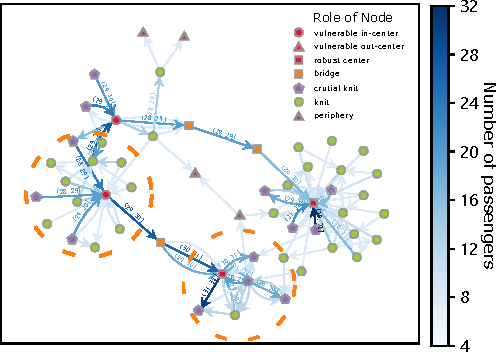
\includegraphics[width=0.7\textwidth]{figs/role_bikesharing.pdf}
  \caption{Role discovery of nodes in the dynamical bikesharing flow network within checking window $T$}\label{fig:role_bikesharing}
\end{figure}

\begin{figure}[!htb]
  \centering
  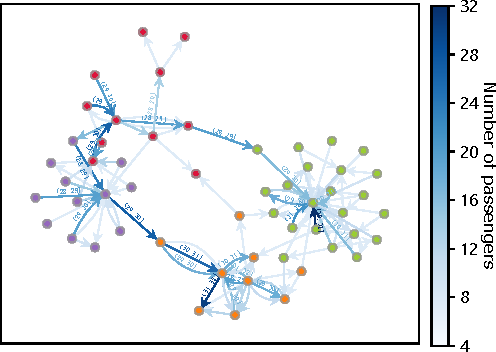
\includegraphics[width=0.7\textwidth]{figs/graph_clustering.pdf}
  \caption{Community detection on the bikesharing flow network within $T$ snapshot}\label{fig:graph_clustering}
\end{figure}

\begin{figure}[!htb]
  \centering
  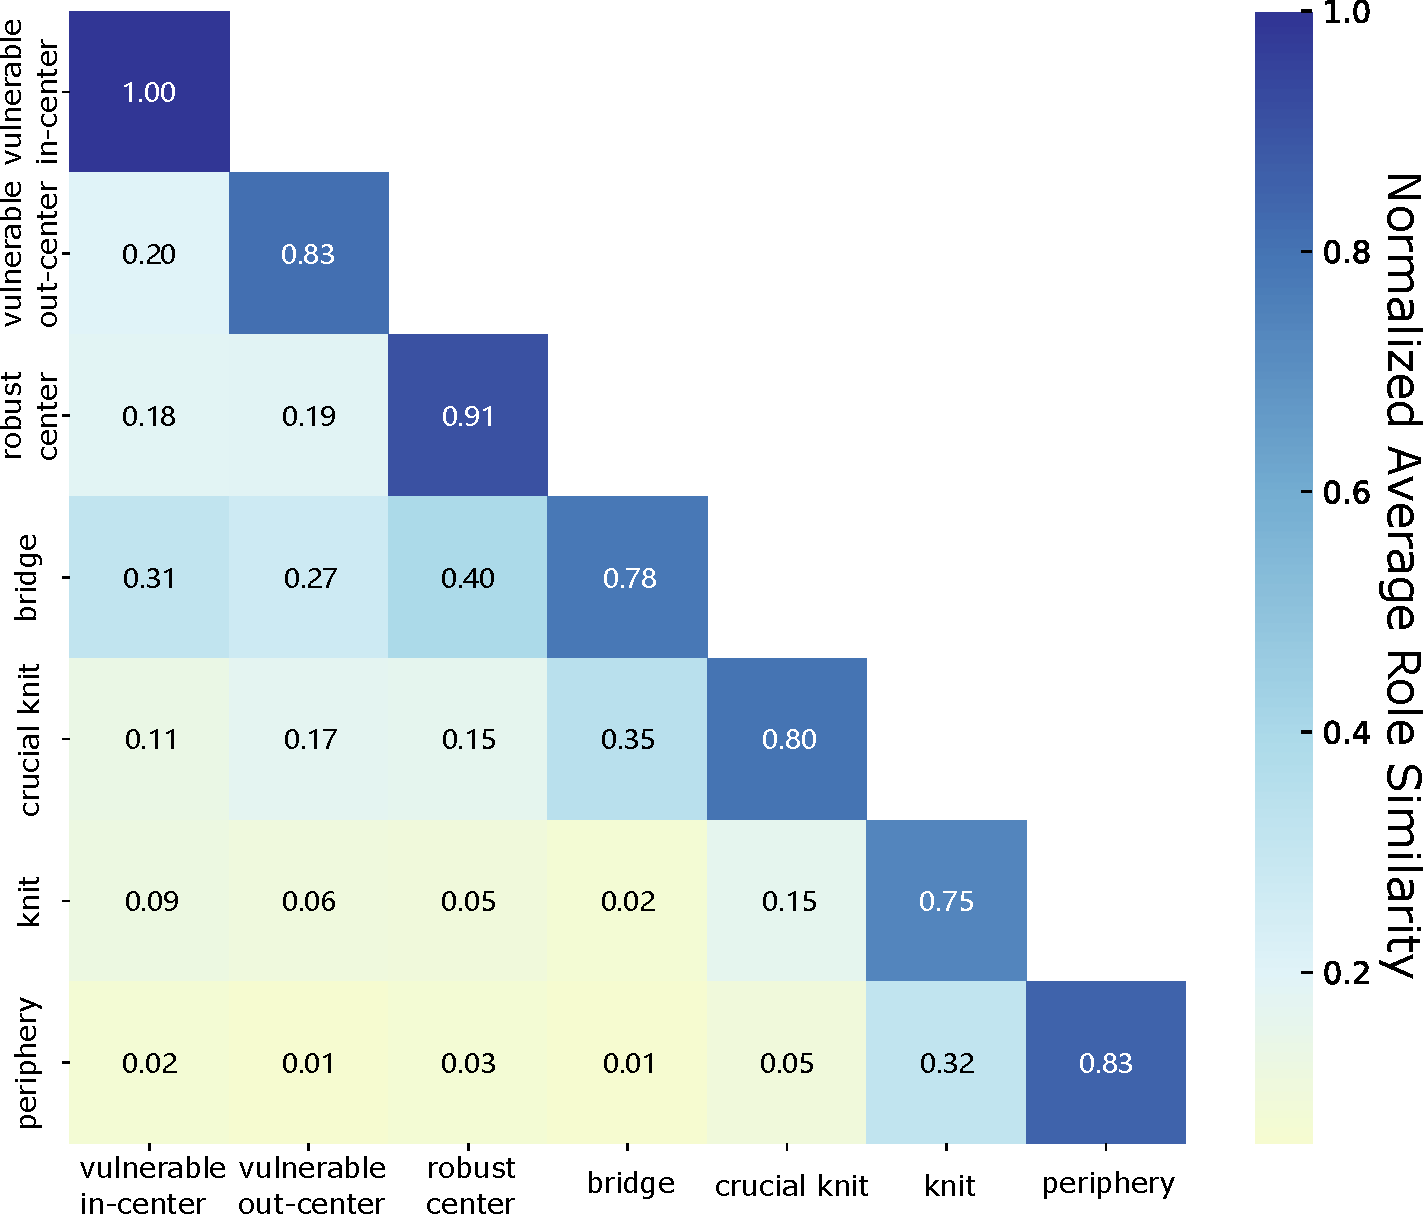
\includegraphics[width=0.7\textwidth]{figs/bikesharing_role_similarity.pdf}
  \caption{Normalized average role similarity matrix of dynamical bikesharing flow networks.}\label{fig:bikesharing_role_similarity}
\end{figure}

As an aside, the concept of roles significantly differs from that of communities. Communities are clusters of nodes with more edges inside the group than outsiders. In contrast, roles are groups of nodes with similar structural features. Community detection is often based on density/cohesion. It is not necessary for nodes of the same role to be in the same community. The comparison between \hyperref[fig:role_bikesharing]{Figure.~\ref{fig:role_bikesharing}} and \hyperref[fig:graph_clustering]{Figure.~\ref{fig:graph_clustering}} presents a concrete example illustrating their differences. In the community detection process, we first assume the concerning dynamical graph is "static" and then implement spectral clustering (\citep{white2005spectral}) to identify communities/clusters. The number of identified communities on the whole network is 32, whereas only 4 clusters are presented in \hyperref[fig:graph_clustering]{Figure.~\ref{fig:graph_clustering}} since the visualized network is just a subgraph of the overall network.

\hyperref[fig:bikesharing_role_similarity]{Figure.~\ref{fig:bikesharing_role_similarity}} shows the normalized average role similarity matrix for bikesharing stations using the cosine function. Squares on the diagonal illustrate intra-group role similarity, whereas the rest of the matrix denotes inter-group similarity. In general, \hyperref[fig:bikesharing_role_similarity]{Figure.~\ref{fig:bikesharing_role_similarity}} illustrates the consistency of clusters of roles, demonstrates the distinguishability of the structural feature matrix $\mathbf{F}$ and the effectiveness of the proposed feature extraction DyReFeX algorithm.

\begin{figure}[!htb]
  \centering
  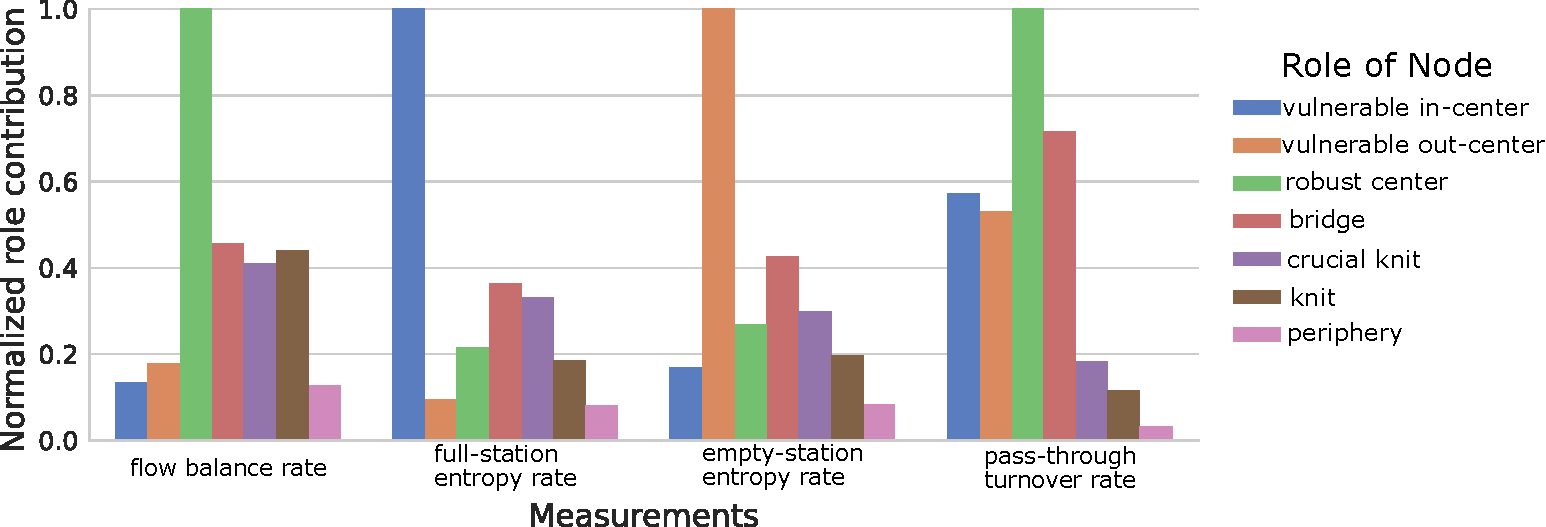
\includegraphics[width=0.95\textwidth]{figs/sense_making.pdf}
  \caption{Station role interpretation in Bikesharing ridership networks}\label{fig:sense_making}
\end{figure}


\begin{figure}[!htb]
  \centering
  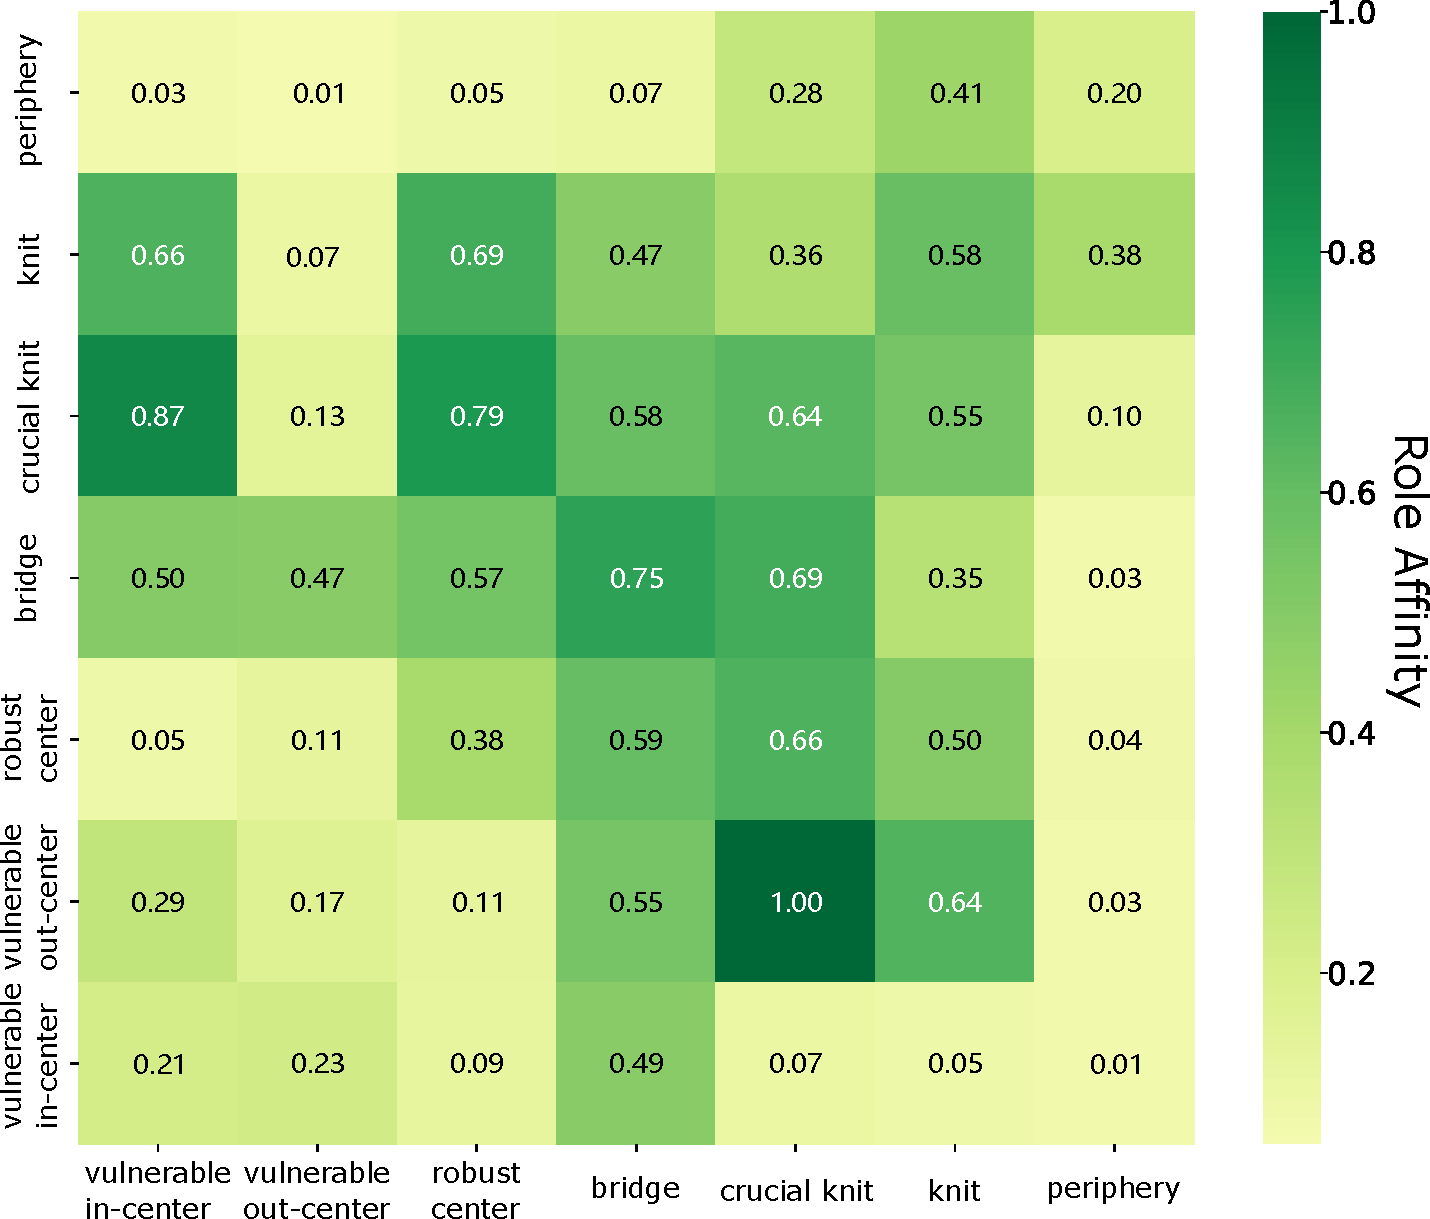
\includegraphics[width=0.7\textwidth]{figs/bikesharing_role_affinity.pdf}
  \caption{Average role affinity matrix of dynamical bikesharing flow network. The x-axis shows the role of destination nodes. The y-axis shows the role of origin nodes.}\label{fig:bikesharing_role_affinity}
\end{figure}


\subsection{Role interpretation of bikesharing stations}
In this subsection, we interpret the roles of bikesharing stations under the context of the dynamical bikesharing flow network in Nanjing based on the methods we discussed in \hyperref[role_inter_method]{Section.\ref{role_inter_method}}. The normalized average role contribution with respect to different service-related measurements and the pair-wise role affinity are presented in \hyperref[fig:role_bikesharing]{Figure.~\ref{fig:sense_making}} and \hyperref[fig:bikesharing_role_affinity]{Figure.~\ref{fig:bikesharing_role_affinity}}, respectively. To recap briefly, role affinity measures the flow weight and network-perspective distance from nodes of one role to nodes of another role.\newline

\noindent \textbullet \, \textbf{Vulnerable in-center (VIC)} has a considerable volume of in-flows. The significant role affinity from nodes of other roles (e.g., bridge, crucial knit, crucial) to VIC nodes presented in \hyperref[fig:bikesharing_role_affinity]{Figure.~\ref{fig:bikesharing_role_affinity}} demonstrates the large in-flows of VIC stations. The low average flow balance rate (AFBR) and high full-station entropy rate (FSER) shown in \hyperref[fig:role_bikesharing]{Figure.~\ref{fig:sense_making}} indicate that VIC stations are susceptible to full-station failure. In other words, VIC stations are highly likely to be full and unlikely to recover from such a service failure, if any happens, during the checking period $T$.\newline

\noindent \textbullet \, \textbf{Vulnerable out-center (VOC)} can be explained in detail in a similar fashion to VIC. In short, a VOC station typically has large out-flows with a high potential to be empty and exhibit irresistibility to such an empty-station state during the evaluating period $T$, as its AFBR and empty-station entropy rate (ESER) indicates.\newline

\noindent \textbullet \, \textbf{Robust centers (RC)} Flows entering and leaving RC stations are both significant. RC stations generally possess a balanced in-out-flow ratio (high AFBR). Also, RC stations exhibit show outstanding robustness in their daily operations. The small FSER and ESER indicate that RC stations tend to recover and be functional again after a service failure. Bicycles returning from users but then rented by others from RC stations have a considerably high turnover rate.\newline

\noindent \textbullet \, \textbf{Crucial knit and knit} Both types of knit stations are members of the clusters with centers to be either VIC, or VOC, or RC. The high role affinity between these knits and network centers (presented in \hyperref[fig:bikesharing_role_affinity]{Figure.~\ref{fig:bikesharing_role_affinity}}) shows consistency with the graph visualization in \hyperref[fig:role_bikesharing]{Figure.~\ref{fig:role_bikesharing}}, further demonstrates (crucial) knits' membership to centers. The difference between them is that crucial knits typically have stronger connectivity with the corresponding center compared to the latter.\newline

\noindent \textbullet \, \textbf{Bridge} stops, as its name implies, connect groups of stations. We found that bridge stations typically have high pass-through bicycle turnover rates, which means there are flows of bikes coming from one cluster of stations to involve in travel transactions in other clusters. For example, a flow pattern leaving one cluster and entering another cluster (the two clusters are circled by dash orange rings) is clearly revealed in \hyperref[fig:role_bikesharing]{Figure.~\ref{fig:role_bikesharing}}\newline

\noindent \textbullet \, \textbf{Periphery} nodes are bikesharing stations with fewer bike flows (sometimes even zero) compared to stops of other roles. As shown in \hyperref[fig:role_bikesharing]{Figure.~\ref{fig:role_bikesharing}} and \hyperref[fig:bikesharing_role_affinity]{Figure.~\ref{fig:bikesharing_role_affinity}}, periphery stations are generally distant to nodes of other roles, except for knits.\newline

To sum up, all three types of centers in the network are essential hubs in terms of bike flow volume and turnover rate. However, VIC and VOC centers could become service bottlenecks for the bikesharing system. Users supposed to return/get a bike to/from VIC and VOC stations have to turn to other bikesharing stops with available bicycles or parking slots. Bridge connects clusters of stations and is also crucial for the system's daily operation. Crucial knit and knit are members of clusters with different degrees of connectivity to centers. Periphery indicates low flows and connectivity to other nodes in the system; thus, it is the least important role. However, we should notice that a bikesharing station may switch among roles over time. We will delve into the role dynamics of stations and explore role variation patterns in the following subsection.

\subsection{Role dynamics of bikesharing stations}
This subsection investigates the role dynamics of individual nodes based on the time-series of role memberships given by W. \hyperref[fig:role_dynamics]{Figure.~\ref{fig:role_dynamics}} shows the within-day and day-to-day role variation behavior of the bikesharing station (colored as the purple node $z$ in \hyperref[fig:d_graph_instance]{Figure.~\ref{fig:d_graph_instance}}) in two weeks (from 2019-03-04 to 2019-03-17). \hyperref[fig:role_dynamics_continue]{Figure.~\ref{fig:role_dynamics_continue} presents the role dynamics solely on 2019-03-04 (Monday) but with a finer time granularity compared to \hyperref[fig:role_dynamics]{Figure.~\ref{fig:role_dynamics}}. Just as before, roles are interpreted by typical node measurements in role contribution bar plots in \hyperref[fig:sense_making]{Figure.~\ref{fig:sense_making}}.

\begin{figure}[!htb]
  \centering
  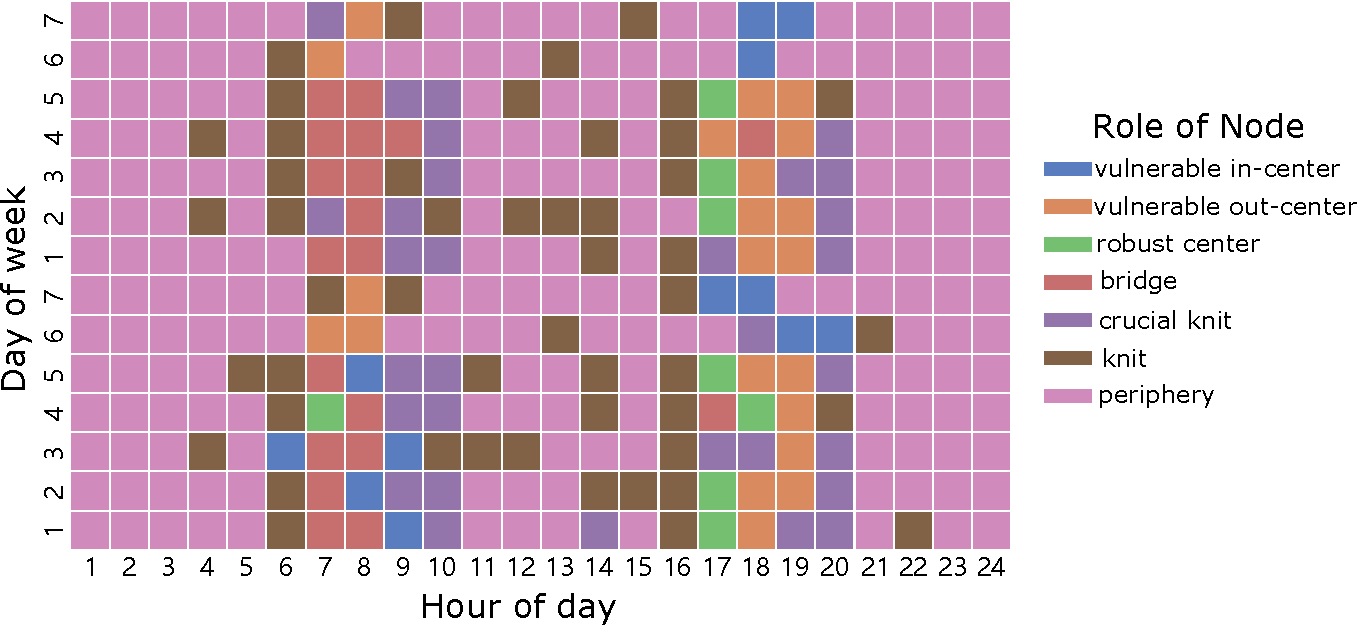
\includegraphics[width=0.85\textwidth]{figs/role_dynamics.pdf}
  \caption{Hourly checking window-based role dynamics matrix of station $v$. The hard role clustering dynamics matrix is transferred from the soft role clustering output $W$ of NMF.}\label{fig:role_dynamics}
\end{figure}

\begin{figure}[!htb]
  \centering
  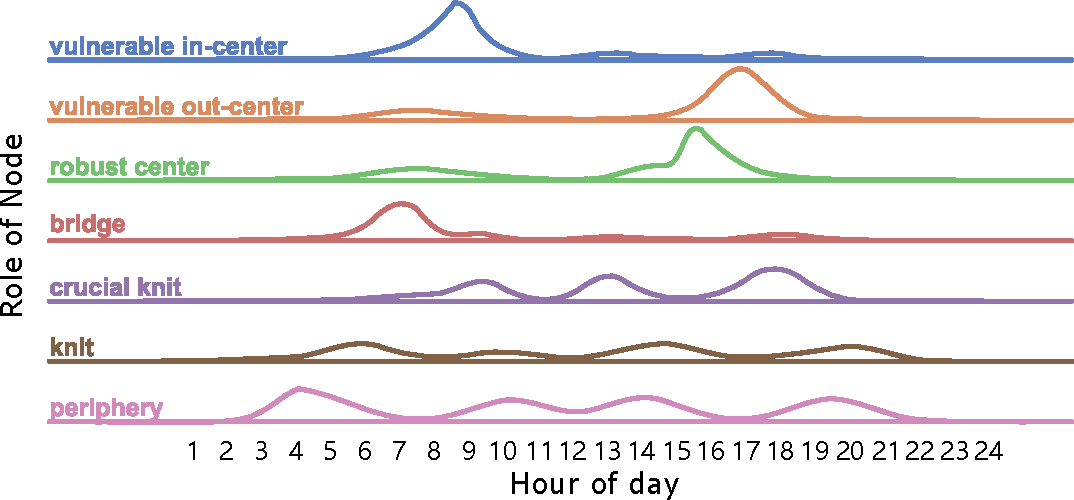
\includegraphics[width=0.8\textwidth]{figs/role_dynamics_continue.pdf}
  \caption{5-minute checking window-based role dynamics of station $v$ based on $W$}.\label{fig:role_dynamics_continue}
\end{figure}

We observe a stationary (but not strictly periodic) behavior of role memberships in \hyperref[fig:role_dynamics]{Figure.~\ref{fig:role_dynamics}} for the concerned bikesharing station $v$. Station $v$ functions as a bridge (sometimes as VIC) in the network from 6 am to 9 am on most weekdays and switches to a crucial knit before noon. Then, $v$ turns into a periphery station in the mid-afternoon when the bikesharing usage decreases.  In the evening rush hours, it becomes either a robust center or VOC and turns into crucial knit or knit when the bikehsharing usage declines again from 7 pm to the end of the day. The appearance of VIC in the morning peak and VOC in the evening peak exposes a loop of large in/out-flows of $v$, suggesting a commuting pattern on weekdays. However, the direction of such a commuting pattern reverses on weekends. Moreover, station $v$ typically serves as a periphery in most periods on weekends since the bikesharing ridership is lower than that on weekdays. Bikesharing operators should optimize their bicycle dispatching schedule accordingly, especially when a considerably consistent (across-day) VOC pattern is unveiled in the evening rush hour in \hyperref[fig:role_dynamics]{Figure.~\ref{fig:role_dynamics}}. However, bikesharing agencies should also pay attention to role variation across days (e.g., the reversed VIC/VOC pattern between weekdays and weekends) and change the bike redistribution plan accordingly. In general, the results shown in \hyperref[fig:role_dynamics_continue]{Figure.~\ref{fig:role_dynamics_continue}} are consistent with the visualization of the first square row in \hyperref[fig:role_dynamics]{Figure.~\ref{fig:role_dynamics}}. \hyperref[fig:role_dynamics]{Figure.~\ref{fig:role_dynamics}} shows the results of role identification based on hourly checking windows. In contrast, we set the checking window every 5 minutes in a day (each checking window's length is still one hour) and output the role dynamics in \hyperref[fig:role_dynamics]{Figure.~\ref{fig:role_dynamics}}. The increasing number of checking windows would enable us to explore role dynamics with a finer granularity. Obviously, there is a trade-off between role investigation granularity and computation cost.

\section{Conclusion}\label{conclusion}
We proposed an efficient framework for automatically extracting roles and mining the role dynamics of nodes in the passenger flow network. Along with the definition of dynamical edge and graph, our novel approach traces flow dynamics and interplay among stations to encode structural information in graphs to feature matrix. We interpret each role with service-related measurements that depicts and evaluates the operating state and efficiency of stations. Network hubs and potential service bottlenecks, which are crucial for operators to maintain or improve the service quality of transit systems, are identified. This helps us answer the question to which station the agencies should pay more attention by inferring the importance of stops. Moreover, we explore role dynamics revealing time-evolving characteristics of stations to answer the question of when a station should be of great concern. We identified stationary and inconsistent role evolution patterns of bikesharing stations, which leads to a deep understanding of how the number, directions, weights of passenger flows, and the topological importance of stations in networks change over time. To our best knowledge, this is the first paper in the academic community to investigate the roles of stations and their dynamics in transportation networks based on node embedding techniques. Our approach is interpretable, feasible to similar transport systems where the O-D matrix is available and lends itself to intuitive visualizations.

The limitation of this study remains: To construct the dynamical passenger flow network, we grouped trips into flows starting and ending in periods/intervals with user-defined length. Decreasing the length of intervals leads to a more complete picture of network dynamics. A trade-off has to be made between the observation granularity and computation cost. We lack methods that can cope with the unique challenges presented by temporal graphs built from travel transactions. Another limitation of this paper is that we only applied our methods to a single-mode passenger flow network. Role identification for a multi-mode graph, such as a bikesharing-bus-metro network, is challenging in modeling and interpretation. However, exploring the time-varting interconnectivity and heterogeneity among various networks is extremely important. 

Despite these limitations, our approach still provides an in-depth insight into the roles of stations and their dynamics in transit systems and contributes to a better understanding of the interplay among transit stations in the network. The role identification of important nodes and potential bottlenecks provides insights for transit agencies to improve service quality. 

\section*{Acknowledgement}
This research is funded by the National Key R\&D Program of China (2018YFB1601300) and the National Natural Science Foundation of China (No.5133800; No.71801041).


%% Loading bibliography style file
%\bibliographystyle{model1-num-names}
\bibliographystyle{cas-model2-names}

% Loading bibliography database
\bibliography{cas-refs}

\end{document}

